\documentclass[border=4pt]{standalone}
\usepackage{amsmath,amssymb}
\usepackage{tikz}
\usetikzlibrary{arrows.meta}
\begin{document}
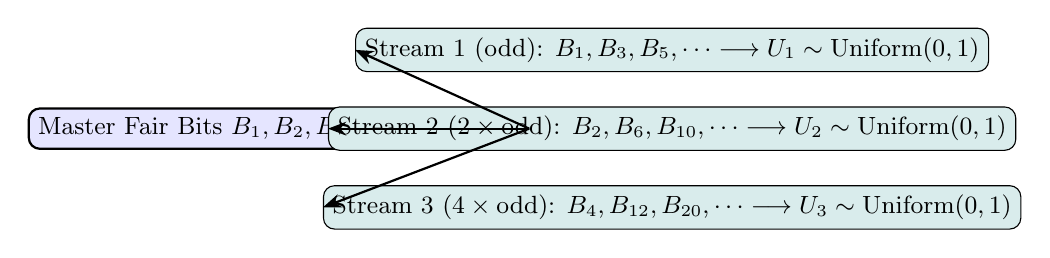
\begin{tikzpicture}[font=\small, >=Stealth]
  \node[draw, thick, fill=blue!10, rounded corners=4pt] (Bits) at (0, 2.0) 
    {Master Fair Bits $B_1, B_2, B_3, B_4, B_5, B_6, \dots$};

  \node[draw, rounded corners, fill=teal!15] (S1) at (5.0, 3.0) 
    {Stream 1 (odd): $B_1, B_3, B_5, \dots \longrightarrow U_1 \sim \mathrm{Uniform}(0,1)$};
  \node[draw, rounded corners, fill=teal!15] (S2) at (5.0, 2.0) 
    {Stream 2 ($2\times\text{odd}$): $B_2, B_6, B_{10}, \dots \longrightarrow U_2 \sim \mathrm{Uniform}(0,1)$};
  \node[draw, rounded corners, fill=teal!15] (S3) at (5.0, 1.0) 
    {Stream 3 ($4\times\text{odd}$): $B_4, B_{12}, B_{20}, \dots \longrightarrow U_3 \sim \mathrm{Uniform}(0,1)$};

  \draw[->, thick] (Bits.east) -- (S1.west);
  \draw[->, thick] (Bits.east) -- (S2.west);
  \draw[->, thick] (Bits.east) -- (S3.west);
\end{tikzpicture}
\end{document}